\documentclass[conference]{IEEEtran}
\IEEEoverridecommandlockouts

\usepackage[T1]{fontenc}
\usepackage{amsmath,amssymb}
\usepackage{graphicx}
\usepackage{booktabs}
\usepackage{xcolor}
\usepackage[hidelinks]{hyperref}
\usepackage{cite}

% Generated by build_numbers.py from results/*.json. Do not edit.
\newcommand{\AdvIllicitAUC}{0.998}
\newcommand{\AdvIllicitClockAUC}{1.000}
\newcommand{\AdvIllicitClockKSShare}{73\%}
\newcommand{\AdvIllicitKSShare}{72\%}
\newcommand{\AdvIllicitN}{169}
\newcommand{\AdvLicitAUC}{0.998}
\newcommand{\AdvLicitClockAUC}{1.000}
\newcommand{\AdvLicitClockKSShare}{10\%}
\newcommand{\AdvLicitKSShare}{7\%}
\newcommand{\AdvLicitN}{6,518}
\newcommand{\ClockAblRFFone}{0.801}
\newcommand{\ClockAblRFFoneDiff}{0.000}
\newcommand{\ClockAblRFFoneP}{=1.00}
\newcommand{\ClockAblRFPRAUCDiff}{0.000}
\newcommand{\ClockAblRFPRAUCP}{=0.84}
\newcommand{\ClockAblXGBFone}{0.800}
\newcommand{\ClockAblXGBFoneDiff}{-0.000}
\newcommand{\ClockAblXGBFoneP}{=0.85}
\newcommand{\ClockAblXGBPRAUCDiff}{0.001}
\newcommand{\ClockAblXGBPRAUCP}{=0.26}
\newcommand{\ClockCount}{5}
\newcommand{\ClockList}{agg\_07, agg\_09, agg\_42, agg\_06, agg\_45}
\newcommand{\ClockMinRho}{0.953}
\newcommand{\DriftDirSAGEPost}{0.016}
\newcommand{\DriftDirSAGEPre}{0.687}
\newcommand{\DriftLogRegPost}{0.066}
\newcommand{\DriftLogRegPre}{0.582}
\newcommand{\DriftMLPPost}{0.031}
\newcommand{\DriftMLPPre}{0.720}
\newcommand{\DriftRFPost}{0.043}
\newcommand{\DriftRFPre}{0.890}
\newcommand{\DriftXGBPost}{0.036}
\newcommand{\DriftXGBPre}{0.888}
\newcommand{\EdaComponents}{49}
\newcommand{\EdaFeaturesAfterFilter}{103}
\newcommand{\EdaHomBase}{9.8\%}
\newcommand{\EdaHomIll}{54.1\%}
\newcommand{\EdaHomLic}{2.4\%}
\newcommand{\EdaIllicitPost}{169}
\newcommand{\EdaIllicitPre}{914}
\newcommand{\EdaIllicitShare}{9.8\%}
\newcommand{\EdaPairsNinetyFive}{96}
\newcommand{\EdaShareTest}{6.5\%}
\newcommand{\EdaShareTrain}{11.6\%}
\newcommand{\GraphDirSAGEgraphFone}{0.669}
\newcommand{\GraphDirSAGEgraphFoneCI}{[0.439,\, 0.757]}
\newcommand{\GraphDirSAGEgraphPRAUC}{0.702}
\newcommand{\GraphGCNgraphFone}{0.515}
\newcommand{\GraphGCNgraphFoneCI}{[0.274,\, 0.644]}
\newcommand{\GraphGCNgraphPRAUC}{0.608}
\newcommand{\GraphPairedRFAFGFoneDiff}{0.014}
\newcommand{\GraphPairedRFAFGFoneP}{<0.001}
\newcommand{\GraphPairedRFAFGNEFoneDiff}{0.007}
\newcommand{\GraphPairedRFAFGNEFoneP}{=0.14}
\newcommand{\GraphPairedRFAFGNEPRAUCDiff}{-0.004}
\newcommand{\GraphPairedRFAFGNEPRAUCP}{=0.003}
\newcommand{\GraphPairedRFAFGPRAUCDiff}{-0.000}
\newcommand{\GraphPairedRFAFGPRAUCP}{=0.19}
\newcommand{\GraphPairedRFAFNEFoneDiff}{0.013}
\newcommand{\GraphPairedRFAFNEFoneP}{<0.001}
\newcommand{\GraphPairedRFAFNEPRAUCDiff}{-0.004}
\newcommand{\GraphPairedRFAFNEPRAUCP}{=0.01}
\newcommand{\GraphPairedRFLFFoneDiff}{-0.061}
\newcommand{\GraphPairedRFLFFoneP}{<0.001}
\newcommand{\GraphPairedRFLFPRAUCDiff}{-0.009}
\newcommand{\GraphPairedRFLFPRAUCP}{<0.001}
\newcommand{\GraphPairedXGBAFGFoneDiff}{-0.009}
\newcommand{\GraphPairedXGBAFGFoneP}{=0.001}
\newcommand{\GraphPairedXGBAFGNEFoneDiff}{0.017}
\newcommand{\GraphPairedXGBAFGNEFoneP}{=0.04}
\newcommand{\GraphPairedXGBAFGNEPRAUCDiff}{-0.003}
\newcommand{\GraphPairedXGBAFGNEPRAUCP}{=0.36}
\newcommand{\GraphPairedXGBAFGPRAUCDiff}{0.002}
\newcommand{\GraphPairedXGBAFGPRAUCP}{=0.04}
\newcommand{\GraphPairedXGBAFNEFoneDiff}{0.014}
\newcommand{\GraphPairedXGBAFNEFoneP}{=0.06}
\newcommand{\GraphPairedXGBAFNEPRAUCDiff}{-0.001}
\newcommand{\GraphPairedXGBAFNEPRAUCP}{=0.77}
\newcommand{\GraphPairedXGBLFFoneDiff}{-0.047}
\newcommand{\GraphPairedXGBLFFoneP}{<0.001}
\newcommand{\GraphPairedXGBLFPRAUCDiff}{-0.015}
\newcommand{\GraphPairedXGBLFPRAUCP}{=0.001}
\newcommand{\GraphRFAFFone}{0.804}
\newcommand{\GraphRFAFFoneCI}{[0.618,\, 0.888]}
\newcommand{\GraphRFAFGFone}{0.813}
\newcommand{\GraphRFAFGFoneCI}{[0.639,\, 0.896]}
\newcommand{\GraphRFAFGNEFone}{0.808}
\newcommand{\GraphRFAFGNEFoneCI}{[0.627,\, 0.890]}
\newcommand{\GraphRFAFGNEPRAUC}{0.789}
\newcommand{\GraphRFAFGPRAUC}{0.793}
\newcommand{\GraphRFAFNEFone}{0.814}
\newcommand{\GraphRFAFNEFoneCI}{[0.636,\, 0.894]}
\newcommand{\GraphRFAFNEPRAUC}{0.789}
\newcommand{\GraphRFAFPRAUC}{0.793}
\newcommand{\GraphRFLFFone}{0.743}
\newcommand{\GraphRFLFFoneCI}{[0.548,\, 0.839]}
\newcommand{\GraphRFLFGFone}{0.748}
\newcommand{\GraphRFLFGFoneCI}{[0.552,\, 0.845]}
\newcommand{\GraphRFLFGPRAUC}{0.785}
\newcommand{\GraphRFLFPRAUC}{0.784}
\newcommand{\GraphSkipGCNgraphFone}{0.507}
\newcommand{\GraphSkipGCNgraphFoneCI}{[0.261,\, 0.639]}
\newcommand{\GraphSkipGCNgraphPRAUC}{0.624}
\newcommand{\GraphXGBAFFone}{0.794}
\newcommand{\GraphXGBAFFoneCI}{[0.613,\, 0.886]}
\newcommand{\GraphXGBAFGFone}{0.787}
\newcommand{\GraphXGBAFGFoneCI}{[0.604,\, 0.878]}
\newcommand{\GraphXGBAFGNEFone}{0.816}
\newcommand{\GraphXGBAFGNEFoneCI}{[0.628,\, 0.896]}
\newcommand{\GraphXGBAFGNEPRAUC}{0.795}
\newcommand{\GraphXGBAFGPRAUC}{0.800}
\newcommand{\GraphXGBAFNEFone}{0.812}
\newcommand{\GraphXGBAFNEFoneCI}{[0.626,\, 0.894]}
\newcommand{\GraphXGBAFNEPRAUC}{0.797}
\newcommand{\GraphXGBAFPRAUC}{0.798}
\newcommand{\GraphXGBLFFone}{0.750}
\newcommand{\GraphXGBLFFoneCI}{[0.568,\, 0.840]}
\newcommand{\GraphXGBLFGFone}{0.749}
\newcommand{\GraphXGBLFGFoneCI}{[0.560,\, 0.841]}
\newcommand{\GraphXGBLFGPRAUC}{0.789}
\newcommand{\GraphXGBLFPRAUC}{0.782}
\newcommand{\HybRFFone}{0.664}
\newcommand{\HybRFFoneDiff}{-0.127}
\newcommand{\HybRFFoneDrop}{0.127}
\newcommand{\HybRFFoneP}{<0.001}
\newcommand{\HybRFPRAUC}{0.696}
\newcommand{\HybXGBFone}{0.662}
\newcommand{\HybXGBFoneDiff}{-0.117}
\newcommand{\HybXGBFoneDrop}{0.117}
\newcommand{\HybXGBFoneP}{=0.001}
\newcommand{\HybXGBPRAUC}{0.692}
\newcommand{\IFAFLicitAnomalousPRAUC}{0.036}
\newcommand{\IFAFLicitAnomalousROCAUC}{0.176}
\newcommand{\IFAFLicitTypicalPRAUC}{0.473}
\newcommand{\IFAFLicitTypicalROCAUC}{0.824}
\newcommand{\IFAFUnsupAnomalousPRAUC}{0.036}
\newcommand{\IFAFUnsupAnomalousROCAUC}{0.170}
\newcommand{\IFAFUnsupTypicalPRAUC}{0.475}
\newcommand{\IFAFUnsupTypicalROCAUC}{0.830}
\newcommand{\IFLFLicitAnomalousPRAUC}{0.037}
\newcommand{\IFLFLicitAnomalousROCAUC}{0.167}
\newcommand{\IFLFLicitTypicalPRAUC}{0.616}
\newcommand{\IFLFLicitTypicalROCAUC}{0.833}
\newcommand{\IFLFUnsupAnomalousPRAUC}{0.038}
\newcommand{\IFLFUnsupAnomalousROCAUC}{0.181}
\newcommand{\IFLFUnsupTypicalPRAUC}{0.374}
\newcommand{\IFLFUnsupTypicalROCAUC}{0.819}
\newcommand{\ImbLRNoneFixedFone}{0.461}
\newcommand{\ImbLRNonePRAUC}{0.319}
\newcommand{\ImbLRNoneTunedFone}{0.515}
\newcommand{\ImbLRSmoteFixedFone}{0.350}
\newcommand{\ImbLRSmotePRAUC}{0.275}
\newcommand{\ImbLRSmoteTunedFone}{0.470}
\newcommand{\ImbLRWeightFixedFone}{0.329}
\newcommand{\ImbLRWeightPRAUC}{0.270}
\newcommand{\ImbLRWeightTunedFone}{0.464}
\newcommand{\ImbMLPNoneFixedFone}{0.620}
\newcommand{\ImbMLPNonePRAUC}{0.605}
\newcommand{\ImbMLPNoneTunedFone}{0.679}
\newcommand{\ImbMLPSmoteFixedFone}{0.620}
\newcommand{\ImbMLPSmotePRAUC}{0.601}
\newcommand{\ImbMLPSmoteTunedFone}{0.651}
\newcommand{\ImbMLPWeightFixedFone}{0.621}
\newcommand{\ImbMLPWeightPRAUC}{0.587}
\newcommand{\ImbMLPWeightTunedFone}{0.640}
\newcommand{\ImbRFNoneFixedFone}{0.827}
\newcommand{\ImbRFNonePRAUC}{0.793}
\newcommand{\ImbRFNoneTunedFone}{0.804}
\newcommand{\ImbRFSmoteFixedFone}{0.798}
\newcommand{\ImbRFSmotePRAUC}{0.807}
\newcommand{\ImbRFSmoteTunedFone}{0.775}
\newcommand{\ImbRFWeightFixedFone}{0.812}
\newcommand{\ImbRFWeightPRAUC}{0.796}
\newcommand{\ImbRFWeightTunedFone}{0.788}
\newcommand{\ImbXGBNoneFixedFone}{0.818}
\newcommand{\ImbXGBNonePRAUC}{0.798}
\newcommand{\ImbXGBNoneTunedFone}{0.794}
\newcommand{\ImbXGBSmoteFixedFone}{0.818}
\newcommand{\ImbXGBSmotePRAUC}{0.816}
\newcommand{\ImbXGBSmoteTunedFone}{0.808}
\newcommand{\ImbXGBWeightFixedFone}{0.805}
\newcommand{\ImbXGBWeightPRAUC}{0.800}
\newcommand{\ImbXGBWeightTunedFone}{0.805}
\newcommand{\LabelEffA}{0.361}
\newcommand{\LabelEffB}{0.385}
\newcommand{\LabelEffC}{0.542}
\newcommand{\LabelEffD}{0.703}
\newcommand{\LabelEffE}{0.714}
\newcommand{\LabelEffF}{0.745}
\newcommand{\LabelEffG}{0.761}
\newcommand{\LabelEffH}{0.768}
\newcommand{\LabelEffI}{0.785}
\newcommand{\LabelEffJ}{0.794}
\newcommand{\LabelEffK}{0.798}
\newcommand{\LabelEffNA}{15}
\newcommand{\LabelEffNB}{30}
\newcommand{\LabelEffNC}{60}
\newcommand{\LabelEffND}{149}
\newcommand{\LabelEffNE}{299}
\newcommand{\LabelEffNF}{598}
\newcommand{\LabelEffNG}{1,495}
\newcommand{\LabelEffNH}{2,989}
\newcommand{\LabelEffNI}{7,474}
\newcommand{\LabelEffNJ}{14,947}
\newcommand{\LabelEffNK}{29,894}
\newcommand{\LabelsFullPRAUC}{0.798}
\newcommand{\LabelsToBeatIF}{60}
\newcommand{\MainLRBudget}{39\%}
\newcommand{\MainLRFone}{0.515}
\newcommand{\MainLRFoneCI}{[0.328,\, 0.626]}
\newcommand{\MainLRPRAUC}{0.319}
\newcommand{\MainLRPRAUCCI}{[0.173,\, 0.443]}
\newcommand{\MainLRPrecision}{0.417}
\newcommand{\MainLRRecall}{0.674}
\newcommand{\MainMLPBudget}{57\%}
\newcommand{\MainMLPFone}{0.679}
\newcommand{\MainMLPFoneCI}{[0.481,\, 0.750]}
\newcommand{\MainMLPPRAUC}{0.605}
\newcommand{\MainMLPPRAUCCI}{[0.425,\, 0.763]}
\newcommand{\MainMLPPrecision}{0.739}
\newcommand{\MainMLPRecall}{0.632}
\newcommand{\MainRFBudget}{61\%}
\newcommand{\MainRFFone}{0.804}
\newcommand{\MainRFFoneCI}{[0.618,\, 0.888]}
\newcommand{\MainRFPRAUC}{0.793}
\newcommand{\MainRFPRAUCCI}{[0.576,\, 0.900]}
\newcommand{\MainRFPrecision}{0.896}
\newcommand{\MainRFRecall}{0.730}
\newcommand{\MainXGBBudget}{62\%}
\newcommand{\MainXGBFone}{0.794}
\newcommand{\MainXGBFoneCI}{[0.613,\, 0.886]}
\newcommand{\MainXGBPRAUC}{0.798}
\newcommand{\MainXGBPRAUCCI}{[0.586,\, 0.903]}
\newcommand{\MainXGBPrecision}{0.865}
\newcommand{\MainXGBRecall}{0.734}
\newcommand{\MemDirSAGERFImp}{99.8\%}
\newcommand{\MemDirSAGETestPRAUC}{0.704}
\newcommand{\MemDirSAGETrainPRAUC}{0.9999}
\newcommand{\MemGCNRFImp}{14.0\%}
\newcommand{\MemGCNTestPRAUC}{0.584}
\newcommand{\MemGCNTrainPRAUC}{0.9797}
\newcommand{\NovelPost}{90\%}
\newcommand{\NovelPre}{31\%}
\newcommand{\PairedXGBLRFoneDiff}{0.284}
\newcommand{\PairedXGBLRFoneP}{<0.001}
\newcommand{\PairedXGBLRPRAUCP}{<0.001}
\newcommand{\PairedXGBMLPFoneDiff}{0.133}
\newcommand{\PairedXGBMLPFoneP}{<0.001}
\newcommand{\PairedXGBMLPPRAUCP}{<0.001}
\newcommand{\PairedXGBRFFoneDiff}{-0.003}
\newcommand{\PairedXGBRFFoneP}{=0.50}
\newcommand{\PairedXGBRFPRAUCP}{=0.07}
\newcommand{\PermAggregated}{0.059}
\newcommand{\PermLocal}{0.695}
\newcommand{\PermStructure}{0.001}
\newcommand{\RepLRAF}{0.449}
\newcommand{\RepLRLF}{0.361}
\newcommand{\RepMLPAF}{0.577}
\newcommand{\RepMLPAFSd}{0.026}
\newcommand{\RepMLPLF}{0.643}
\newcommand{\RepMLPLFSd}{0.036}
\newcommand{\RepRFAF}{0.810}
\newcommand{\RepRFAFSd}{0.005}
\newcommand{\RepRFLF}{0.778}
\newcommand{\RepRFLFSd}{0.008}
\newcommand{\ShapAgg}{35\%}
\newcommand{\ShapLocal}{62\%}
\newcommand{\ShapStruct}{3\%}
\newcommand{\ShapTopFeature}{local\_52}
\newcommand{\UnsBaseRate}{0.065}
\newcommand{\WFExpandingPost}{0.185}
\newcommand{\WFExpandingPre}{0.905}
\newcommand{\WFSlidingPost}{0.144}
\newcommand{\WFSlidingPre}{0.896}
\newcommand{\WFStaticPost}{0.043}
\newcommand{\WFStaticPre}{0.890}


\begin{document}

\title{Detecting Illicit Bitcoin Transactions:\\
Graphs, Imbalance and Drift on the Elliptic Dataset}

\author{\IEEEauthorblockN{Anes Berbi\'c}
\IEEEauthorblockA{International University of Sarajevo\\
EE418 Machine Learning, Student ID 210302141}}

\maketitle

\begin{abstract}
We study illicit transaction detection on the Elliptic Bitcoin dataset (203,769
transactions, 49 time steps). After reproducing the published baselines, we
rebuild the evaluation so that hyper-parameters and thresholds are chosen on
time-ordered validation folds only, every model runs with five seeds, and every
result carries a block-bootstrap confidence interval over time steps. Random
Forest and XGBoost are statistically tied (illicit F1 \MainRFFone{} and
\MainXGBFone{}). The transaction graph helps mainly through neighbour-aggregated
features (+0.06 F1); structural features and GNN embeddings add at most 0.02 F1
and no PR-AUC. A directed GNN we propose beats GCN by about 0.15 F1 but stays below
the trees, and appending its embeddings to a tree model \emph{lowers} F1 by
0.12 because the GNN memorises its training labels. Isolation Forest ranks
transactions worse than random: illicit transactions are typical, not anomalous;
inverting its score yields PR-AUC \IFAFUnsupTypicalPRAUC{} without labels.
Finally, we explain why all models fail after a dark market shutdown: after it,
\NovelPost{} of illicit transactions lie closer to licit than to known illicit
activity, and retraining before every step recovers little.
\end{abstract}

\section{Introduction}

Bitcoin transactions are public, but the people behind them are not. That
combination makes the blockchain attractive for ransomware payments, darknet
markets and laundering, and it also gives investigators a complete record to
search. The question is how to search it. A compliance team cannot review
every transaction, so it needs a model that ranks them by how suspicious they
are and that keeps working as criminals change their behaviour.

The Elliptic Data Set~\cite{weber2019} is the standard public benchmark for
this problem: 203,769 real Bitcoin transactions over 49 time steps, of which
4,545 are labelled illicit and 42,019 licit, linked by 234,355 payment flows.
Weber et al.\ found that a Random Forest on the tabular features beat a Graph
Convolutional Network (GCN), and that \emph{every} model stopped detecting
illicit activity after a dark market was shut down at time step 43.

This project asks: \emph{can we tell illicit Bitcoin transactions apart from
licit ones, using their features and their position in the transaction graph?}
We answer it in five parts, each with a protocol designed to avoid the ways a
study on this dataset can fool itself.

\begin{enumerate}
  \item \textbf{Reproduction.} We first re-run the published baselines on the
        published split. Matching them is what makes everything after it credible.
  \item \textbf{A fair model comparison.} Hyper-parameters and decision
        thresholds are chosen on time-ordered validation folds only; every model
        runs with five seeds; every result has a confidence interval that
        respects the time structure, and model differences are tested.
  \item \textbf{Does the graph help?} We compare tabular features, label-free
        graph statistics, three graph neural networks (including a directed
        variant we motivate from the data) and the hybrid of GNN embeddings
        with a tree model.
  \item \textbf{Without labels.} We measure whether illicit transactions stand
        out as anomalies, and how many labels a supervised model needs before it
        beats the label-free detector.
  \item \textbf{Why models fail over time.} We show what changed after the dark
        market shutdown, whether the new illicit transactions resemble anything
        seen in training, and whether retraining fixes it.
\end{enumerate}

All code, results and figures are reproducible with one command from the
public repository.\footnote{\url{https://github.com/berbicanes/EllipticML}}

\section{Related Work}

\textbf{The Elliptic benchmark.} Weber et al.~\cite{weber2019} released the
dataset with a temporal split (time steps 1--34 for training, 35--49 for
testing) and compared Logistic Regression, Random Forest, an MLP and GCNs.
Random Forest on all features reached an illicit F1 of 0.788; concatenating GCN
node embeddings to the features raised it to 0.796. The best pure graph model,
EvolveGCN~\cite{pareja2020}, reached 0.720. They also reported that even a
Random Forest retrained after every test step could not recover after the dark
market shutdown. Elmougy and Liu~\cite{elmougy2023} extended the data with
wallet addresses and further features (Elliptic++).

\textbf{Graph neural networks.} The GCN~\cite{kipf2017} propagates node
features over a symmetric, degree-normalised adjacency matrix. GraphSAGE
\cite{hamilton2017} keeps a separate weight for a node's own representation and
for its aggregated neighbours. Rossi et al.~\cite{rossi2023} showed that
treating in- and out-edges separately helps on graphs where neighbours tend to
have \emph{different} labels; we adopt this idea for payment flows, which are
inherently directed.

\textbf{Imbalanced classification.} With 2--10\% positives, accuracy and ROC-AUC
are misleading; the precision--recall curve is more informative
\cite{saito2015}. SMOTE~\cite{chawla2002} creates synthetic minority samples;
class weights re-balance the loss. For F1, the optimal decision threshold is
generally not 0.5 and should be chosen on held-out data~\cite{lipton2014}.

\textbf{Anomaly detection and drift.} Isolation Forest~\cite{liu2008} scores
points by how easily random splits isolate them, without labels. Concept drift,
a change in the joint distribution of features and labels over time, is the
central obstacle for deployed fraud models~\cite{gama2014}.

\textbf{Uncertainty.} When observations come in dependent blocks, the bootstrap
should resample whole blocks~\cite{kunsch1989}. Transactions of the same time
step share a market regime and graph, so we resample time steps.

\section{Data}

\textbf{Structure.} Each of the 203,769 nodes is a transaction with a time step
(1--49, about two weeks each) and 165 anonymised features: 93 \emph{local}
features describing the transaction itself (inputs, outputs, fees, amounts, \dots)
and 72 \emph{aggregated} features, statistics of the same quantities over its
one-hop neighbours. Each of the 234,355 directed edges is a flow of bitcoin from
one transaction to another. 77\% of nodes are unlabelled; of the labelled ones,
\EdaIllicitShare{} are illicit.

\textbf{Every time step is a separate graph.} No edge connects two time steps,
and each step forms exactly one connected component (\EdaComponents{} weak
components for 49 steps). This has two consequences we rely on later: graph
statistics computed on the whole graph never mix information across time, and a
graph neural network trained on the full graph cannot pass messages from test
steps to training steps.

\begin{figure}[t]
  \centering
  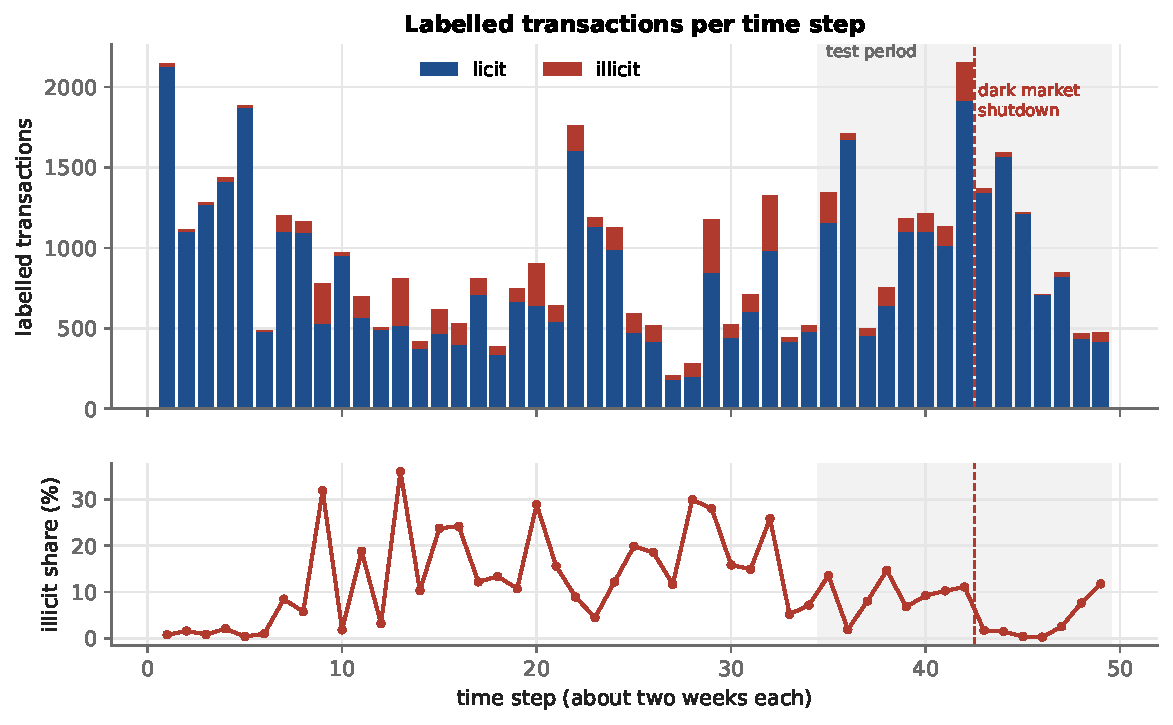
\includegraphics[width=\columnwidth]{../reports/figures/eda_labels_over_time.pdf}
  \caption{Labelled transactions per time step. The illicit share moves between
  0\% and 36\% and falls after the dark market shutdown (dashed line).
  Grey: test period.}
  \label{fig:labels}
\end{figure}

\textbf{Imbalance and its movement over time.} Fig.~\ref{fig:labels} shows that
the illicit share is far from stable: \EdaShareTrain{} in the training steps,
\EdaShareTest{} in the test steps, and almost zero in steps 43--46. Only
\EdaIllicitPost{} illicit transactions occur in steps 43--49, against
\EdaIllicitPre{} in steps 35--42, so the second half of the test period carries
little weight in any pooled metric, and per-step results there are noisy.

\textbf{Redundancy.} \EdaPairsNinetyFive{} feature pairs have $|r|>0.95$; a greedy
filter at that level keeps \EdaFeaturesAfterFilter{} of 165 features
(Fig.~\ref{fig:corr}). Tree ensembles are insensitive to this
redundancy; for the linear model and the MLP we use $L_2$ regularisation instead
of discarding features. In a two-dimensional PCA view (Fig.~\ref{fig:pca}) the
illicit transactions lie inside the licit cloud: no linear projection separates
them, which anticipates the weak result of Logistic Regression.

\begin{figure}[t]
  \centering
  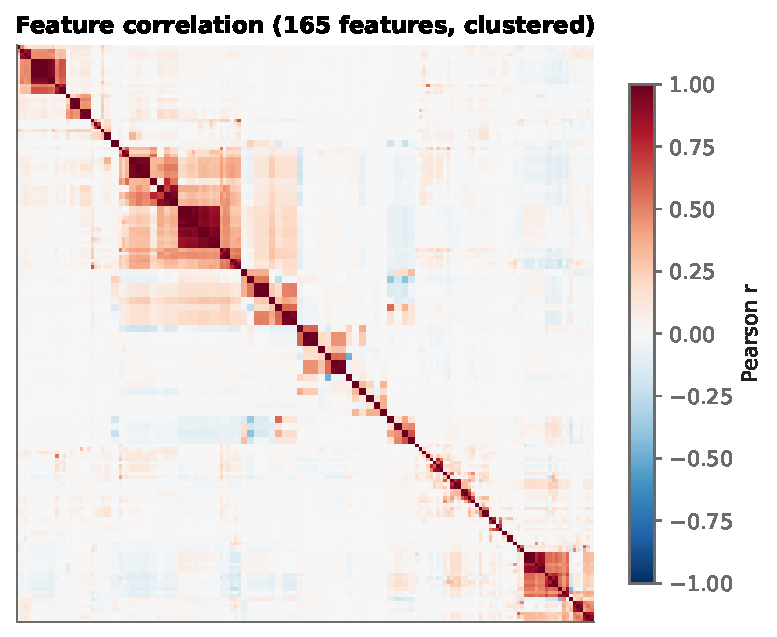
\includegraphics[width=0.78\columnwidth]{../reports/figures/eda_feature_correlation.pdf}
  \caption{Pearson correlation of the 165 features, hierarchically clustered.}
  \label{fig:corr}
\end{figure}

\begin{figure}[t]
  \centering
  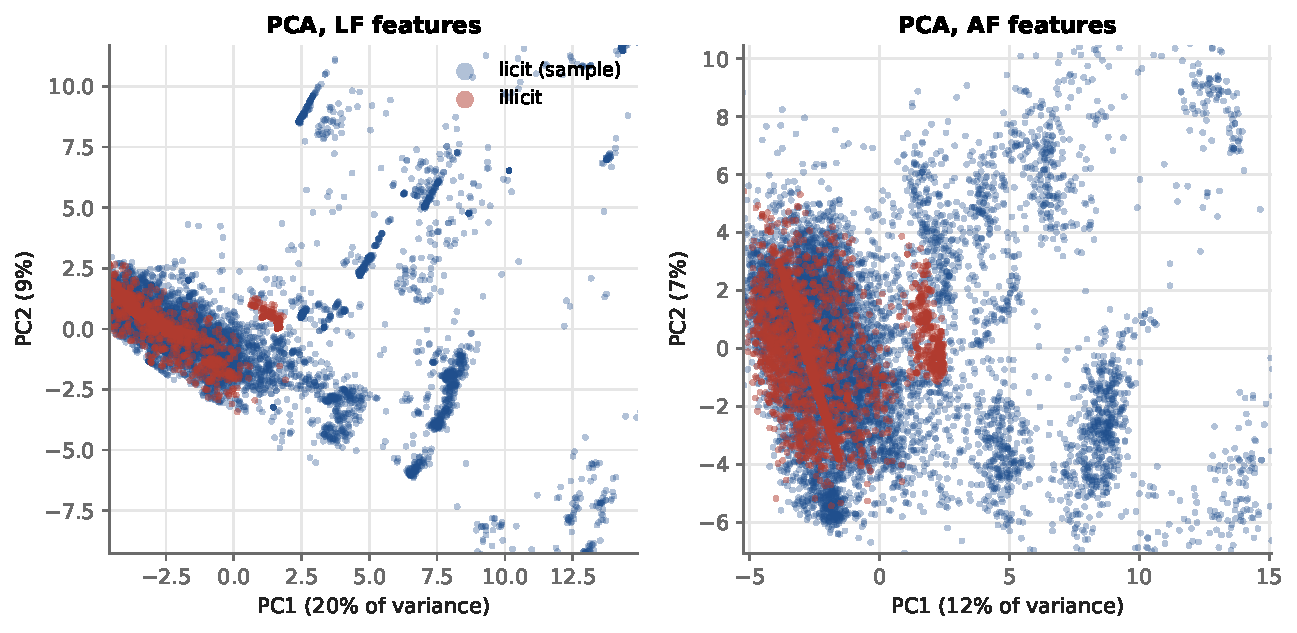
\includegraphics[width=\columnwidth]{../reports/figures/eda_pca.pdf}
  \caption{First two principal components of local (LF) and all (AF) features
  (licit transactions subsampled).}
  \label{fig:pca}
\end{figure}

\textbf{The graph carries label information.} Of the labelled neighbours of an
illicit transaction, \EdaHomIll{} are illicit, against \EdaHomLic{} for a licit
transaction (base rate \EdaHomBase{}). Illicit transactions cluster in the graph.
Their shape also differs (Fig.~\ref{fig:degree}): no illicit transaction has more
than three outputs, while licit ones reach hundreds, yet some illicit
transactions collect up to $\sim$180 inputs. Direction matters, which motivates
the directed GNN of Section~\ref{sec:method}.

\begin{figure}[t]
  \centering
  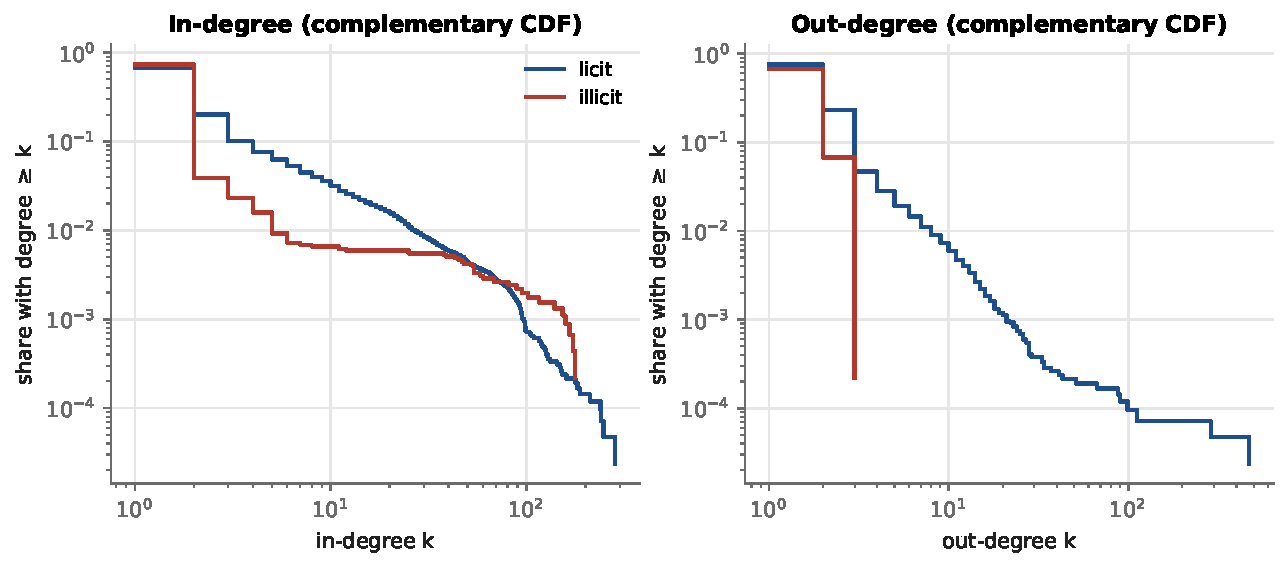
\includegraphics[width=\columnwidth]{../reports/figures/eda_degree.pdf}
  \caption{Degree distributions (share of transactions with degree $\geq k$).
  Illicit transactions never have more than three outputs.}
  \label{fig:degree}
\end{figure}

\section{Method}
\label{sec:method}

\subsection{Evaluation protocol}

\textbf{Split.} We keep the split of Weber et al.: labelled transactions of steps
1--34 (29,894 rows) for training, steps 35--49 (16,670 rows) for testing.
Unlabelled rows are never used by a supervised model. A random split would place
transactions from the same two weeks, and from the future, on both sides.

\textbf{Validation without touching the test set.} All choices are made on
\emph{expanding-window folds} inside the training period: the validation blocks
are steps 20--22, 23--25, 26--28, 29--31 and 32--34, and each fold trains on all
steps before its block. Hyper-parameters are chosen by mean validation PR-AUC.
The decision threshold is then the one that maximises F1 on the pooled
out-of-fold predictions~\cite{lipton2014}. The final model is refit on steps
1--34 and applied once to the test steps.

\textbf{No time step as a feature.} Weber et al.\ include the time step among the
local features. Under a temporal split every test value lies outside the
training range, so the column can only mislead. In our reproduction, removing it
raised Logistic Regression's F1 on local features from 0.36 to 0.51. We keep it
only where we reproduce the paper.

\textbf{Leakage guards.} Scaling and SMOTE live inside the model pipeline and are
refit on every training fold. Graph features use the edge list only, never labels.
Unit tests assert that no test step and no future step ever reaches training.

\textbf{Metrics.} The positive class is \emph{illicit}. We report precision,
recall and F1 at the chosen threshold, PR-AUC (average precision, threshold-free
and the most informative single number under imbalance~\cite{saito2015}),
ROC-AUC, and an \emph{analyst budget} metric: the share of all illicit test
transactions caught if an analyst reviews the 100 highest-scored transactions of
every time step.

\textbf{Uncertainty.} Each stochastic model runs with five seeds. For confidence
intervals we average the five seeds' scores and draw 1,000 bootstrap samples of
\emph{time steps} (not rows): a resample is 15 test steps drawn with replacement,
each bringing all of its transactions~\cite{kunsch1989}. Two models are compared
with a paired bootstrap (2,000 samples) on the same resampled steps; the p-value
is twice the share of resamples in which the difference changes sign.

\subsection{Models}

\textbf{Tabular.} Logistic Regression ($L_2$, standardised inputs), Random
Forest~\cite{breiman2001}, XGBoost~\cite{chen2016} and an MLP (PyTorch, Adam).
Search spaces: LR $C\in\{0.01,0.1,1,10\}$; RF 500 trees, max features
$\in\{\sqrt{d}, 0.3d, 50\}$, min leaf size $\in\{1,3\}$; XGBoost 600 rounds,
depth $\in\{4,6,8\}$, learning rate $\in\{0.03, 0.1\}$; MLP hidden layers
$\in\{(50),(128,64)\}$, dropout $\in\{0,0.2\}$, weight decay $\in\{0,10^{-4}\}$.

\textbf{Imbalance strategies.} \emph{None}, \emph{class weights} (inverse class
frequency) and \emph{SMOTE}~\cite{chawla2002} on training folds only, each with
the fixed 0.5 threshold and with the tuned threshold.

\textbf{Graph structure features (G).} Nine label-free statistics per
transaction: in- and out-degree, number of transactions reachable within two hops
upstream and downstream, mean and maximum neighbour degree, local clustering
coefficient, and PageRank~\cite{page1999} on the graph and on its reverse.

\textbf{Graph neural networks.} All three are trained full-batch on the whole
graph with a weighted cross-entropy (0.3 licit / 0.7 illicit, as
in~\cite{weber2019}) on labelled training nodes.
\begin{itemize}
  \item \textbf{GCN}~\cite{kipf2017}: $H=\mathrm{ReLU}(\hat{A}XW_0)$,
        logits $=\hat{A}HW_1$, with $\hat{A}=D^{-1/2}(A+A^\top+I)D^{-1/2}$.
  \item \textbf{Skip-GCN}~\cite{weber2019}: GCN plus a linear skip connection
        from the raw features to the output.
  \item \textbf{DirSAGE} (ours, after~\cite{hamilton2017,rossi2023}): two
        layers of $h_v' = \mathrm{ReLU}(W_s h_v + W_{in}\,\overline{h}_{N^{in}(v)}
        + W_{out}\,\overline{h}_{N^{out}(v)})$, where $\overline{h}$ is the mean
        over senders or receivers. Unlike the GCN, it can tell its own features
        from its neighbours' and senders from receivers. A unit test with a
        synthetic graph shows the GCN failing exactly this distinction.
\end{itemize}
Configuration (learning rate $\in\{10^{-3}, 3\cdot10^{-3}\}$, dropout
$\in\{0,0.3\}$) and epoch count (up to 1,000, checked every 25) are chosen by
PR-AUC on steps 30--34 after training on 1--29; the threshold is F1-optimal on
the same steps. Because no edge crosses time steps, the test graphs are
disconnected from the training graphs, and full-graph training leaks nothing.

\textbf{Hybrid (NE).} Following~\cite{weber2019}, the 100-dimensional hidden
layer of the GCN is appended to the features of a tree model.

\textbf{Unsupervised.} Isolation Forest~\cite{liu2008} (500 trees, 4,096 samples
per tree) fitted on \emph{all} 136,265 transactions of steps 1--34, labelled or
not, without using any label; and, as a semi-supervised middle ground, on known
licit transactions only.

\section{Results}

\subsection{Reproducing the published baselines (E1)}

With the paper's split, feature sets (including the time step) and stated
hyper-parameters, our Random Forest reaches an illicit F1 of \RepRFAF{}
($\pm$\RepRFAFSd{} over five seeds) on all features, against 0.788 published
(Fig.~\ref{fig:repro}). On local features we obtain \RepRFLF{}, above the
published 0.694. The MLP on local features matches (\RepMLPLF{} vs 0.649); on all
features it is lower (\RepMLPAF{} vs 0.653), a gap we attribute to unreported
training details (batch size, initialisation, input scaling). Logistic
Regression stays below the paper (\RepLRAF{} vs 0.481) even with the 2019
scikit-learn defaults. The ranking of models, which is what the paper's
conclusions rest on, is reproduced: Random Forest $>$ MLP $>$ Logistic Regression.

\begin{figure}[t]
  \centering
  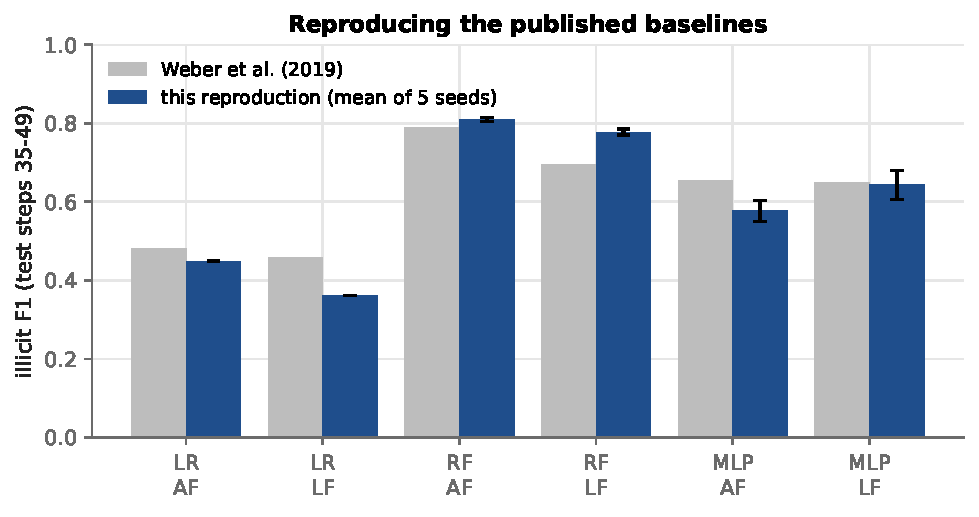
\includegraphics[width=\columnwidth]{../reports/figures/e01_reproduction.pdf}
  \caption{Illicit F1 of the published baselines~\cite{weber2019} and of our
  reproduction (mean and standard deviation over five seeds).}
  \label{fig:repro}
\end{figure}

\subsection{Model comparison under a fair protocol (E2)}

Table~\ref{tab:main} gives the main comparison on all 165 features without
the time step, with tuned hyper-parameters and validation-chosen thresholds.
Random Forest (F1 \MainRFFone{}) and XGBoost (\MainXGBFone{}) are
\emph{statistically tied}: the paired bootstrap gives $p\PairedXGBRFFoneP{}$ for
F1 and $p\PairedXGBRFPRAUCP{}$ for PR-AUC. Both are clearly better than the MLP
(\MainMLPFone{}) and Logistic Regression (\MainLRFone{}), with $p<0.001$.

\begin{table}[t]
  \centering
  \caption{Test results (steps 35--49), mean of five seeds. CIs are 95\%
  block-bootstrap intervals over time steps. Budget: share of illicit
  transactions found by reviewing the top 100 per step.}
  \label{tab:main}
  \setlength{\tabcolsep}{3pt}
  \footnotesize
  \begin{tabular}{lcccc}
    \toprule
    Model & F1 [95\% CI] & PR-AUC [95\% CI] & Prec. / Rec. & Budget \\
    \midrule
    RF      & \MainRFFone{}  {\scriptsize\MainRFFoneCI{}}  & \MainRFPRAUC{}  {\scriptsize\MainRFPRAUCCI{}}  & \MainRFPrecision{} / \MainRFRecall{}   & \MainRFBudget{} \\
    XGBoost & \MainXGBFone{} {\scriptsize\MainXGBFoneCI{}} & \MainXGBPRAUC{} {\scriptsize\MainXGBPRAUCCI{}} & \MainXGBPrecision{} / \MainXGBRecall{} & \MainXGBBudget{} \\
    MLP     & \MainMLPFone{} {\scriptsize\MainMLPFoneCI{}} & \MainMLPPRAUC{} {\scriptsize\MainMLPPRAUCCI{}} & \MainMLPPrecision{} / \MainMLPRecall{} & \MainMLPBudget{} \\
    LR      & \MainLRFone{}  {\scriptsize\MainLRFoneCI{}}  & \MainLRPRAUC{}  {\scriptsize\MainLRPRAUCCI{}}  & \MainLRPrecision{} / \MainLRRecall{}   & \MainLRBudget{} \\
    \bottomrule
  \end{tabular}
\end{table}

The confidence intervals are the most sobering part of the table. The interval
for the best F1 spans more than 0.25. The test period contains 15 time steps,
not 16,670 independent transactions, and the steps differ wildly in difficulty
(Section~\ref{sec:drift}). Differences of a few hundredths between models, the
scale at which much of the literature on this dataset ranks methods, are well
inside this uncertainty unless tested with a paired design as we do here.

\subsection{Handling the imbalance (E3)}

Fig.~\ref{fig:imbalance} crosses three training strategies with two
threshold rules. Three findings stand out.

\emph{Re-balancing does not make the strong models rank better.} For Random
Forest and XGBoost, class weights and SMOTE change PR-AUC by about one point at
most (XGBoost: \ImbXGBNonePRAUC{} without, \ImbXGBSmotePRAUC{} with SMOTE). For
Logistic Regression and the MLP they make it slightly worse.

\emph{Re-balancing mostly moves the decision boundary.} At the fixed 0.5
threshold, class weights and SMOTE push Logistic Regression towards
high recall and very low precision (F1 \ImbLRNoneFixedFone{} $\rightarrow$
\ImbLRWeightFixedFone{}). The same shift is available, more cleanly, by choosing
the threshold.

\emph{Threshold tuning helps weak models but not the trees.} A tuned threshold
lifts Logistic Regression from \ImbLRNoneFixedFone{} to \ImbLRNoneTunedFone{}
and the MLP from \ImbMLPNoneFixedFone{} to \ImbMLPNoneTunedFone{}. For the Random
Forest, the threshold tuned on validation steps is \emph{worse} than 0.5
(\ImbRFNoneTunedFone{} vs \ImbRFNoneFixedFone{}). The best threshold moves over
time: it is a property of the period, not of the model. We still report tuned
thresholds as the main result, because 0.5 being better is only visible in
hindsight.

\begin{figure}[t]
  \centering
  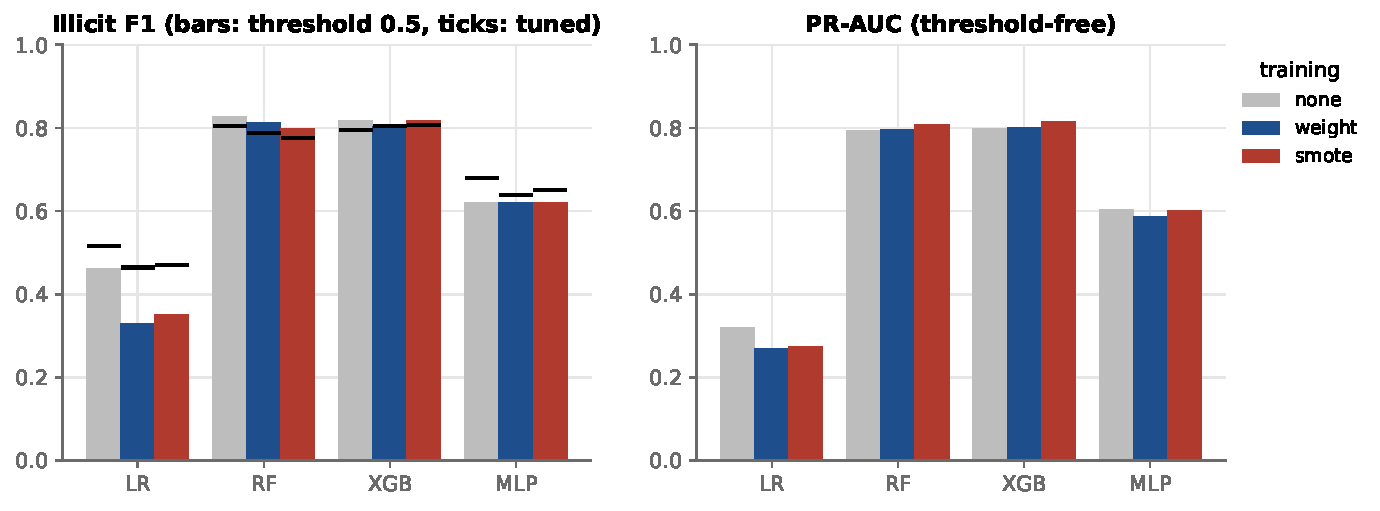
\includegraphics[width=\columnwidth]{../reports/figures/e03_imbalance.pdf}
  \caption{Imbalance strategies. Left: illicit F1 at threshold 0.5 (bars) and at
  the validation-tuned threshold (ticks). Right: PR-AUC. Mean of five seeds.}
  \label{fig:imbalance}
\end{figure}

\subsection{Does the graph help? (E4, E5)}

Fig.~\ref{fig:graph} answers the research question in
three steps.

\emph{Information about the neighbourhood helps, clearly.} Adding the 72
aggregated neighbour features to the 93 local ones raises F1 from
\GraphRFLFFone{} to \GraphRFAFFone{} for Random Forest and from
\GraphXGBLFFone{} to \GraphXGBAFFone{} for XGBoost ($p<0.001$ in the paired test
for both). A transaction's position in the graph, summarised by its neighbours'
features, carries signal its own features do not.

\emph{Anything beyond that adds little.} The nine structural features (G) and the
GCN embeddings (NE) change F1 by at most two hundredths: Random Forest gains
\GraphPairedRFAFGFoneDiff{} with G ($p\GraphPairedRFAFGFoneP{}$) and XGBoost
\GraphPairedXGBAFGNEFoneDiff{} with G and NE together
($p\GraphPairedXGBAFGNEFoneP{}$), while G alone changes XGBoost's F1 by
\GraphPairedXGBAFGFoneDiff{}. PR-AUC moves by less than 0.005 in
every case, so these features shift the precision--recall trade-off at the
chosen threshold rather than improving the ranking. This matches the
+0.008 Weber et al.\ reported for NE and is consistent with E8: the
structural features carry under 3\% of the model's attribution.

\emph{Graph neural networks alone are not competitive, but direction matters.}
The GCN reaches F1 \GraphGCNgraphFone{} and Skip-GCN
\GraphSkipGCNgraphFone{}, below the published 0.628 and 0.705; with our
validation-chosen thresholds both trade recall for precision. Our directed DirSAGE reaches
\GraphDirSAGEgraphFone{} (PR-AUC \GraphDirSAGEgraphPRAUC{} against
\GraphGCNgraphPRAUC{}), the largest improvement from any single design choice
in this study, and it follows directly from the EDA: payment flows are directed
and illicit transactions have a distinctive in/out shape, which a symmetric GCN
cannot see. It still trails the tree models by more than 0.1 F1.

\emph{A stronger GNN makes a worse hybrid (E5).} If GCN embeddings help a
little, should the better DirSAGE embeddings help more? They do the opposite:
appended to AF they \emph{lower} F1 by \HybRFFoneDrop{} for Random Forest and
\HybXGBFoneDrop{} for XGBoost ($p\HybRFFoneP{}$). The diagnostic in
Table~\ref{tab:memo} explains why. The embeddings come from a GNN trained on the
labels of steps 1--34, and DirSAGE has memorised them: its PR-AUC on training
rows is \MemDirSAGETrainPRAUC{}, against \MemDirSAGETestPRAUC{} on test rows. The
Random Forest sees an almost perfect feature during training and puts
\MemDirSAGERFImp{} of its importance on it, so at test time it is only as good
as DirSAGE. The GCN overfits less, and the forest gives its embeddings only
\MemGCNRFImp{}. The published hybrid works \emph{because} its GNN is weak; a
correct hybrid would need embeddings produced out-of-fold.

\begin{table}[t]
  \centering
  \caption{Why DirSAGE embeddings hurt the hybrid (E5b, seed 0).}
  \label{tab:memo}
  \footnotesize
  \begin{tabular}{lccc}
    \toprule
    GNN & PR-AUC train & PR-AUC test & RF importance on NE \\
    \midrule
    GCN     & \MemGCNTrainPRAUC{}     & \MemGCNTestPRAUC{}     & \MemGCNRFImp{} \\
    DirSAGE & \MemDirSAGETrainPRAUC{} & \MemDirSAGETestPRAUC{} & \MemDirSAGERFImp{} \\
    \bottomrule
  \end{tabular}
\end{table}

\begin{figure}[t]
  \centering
  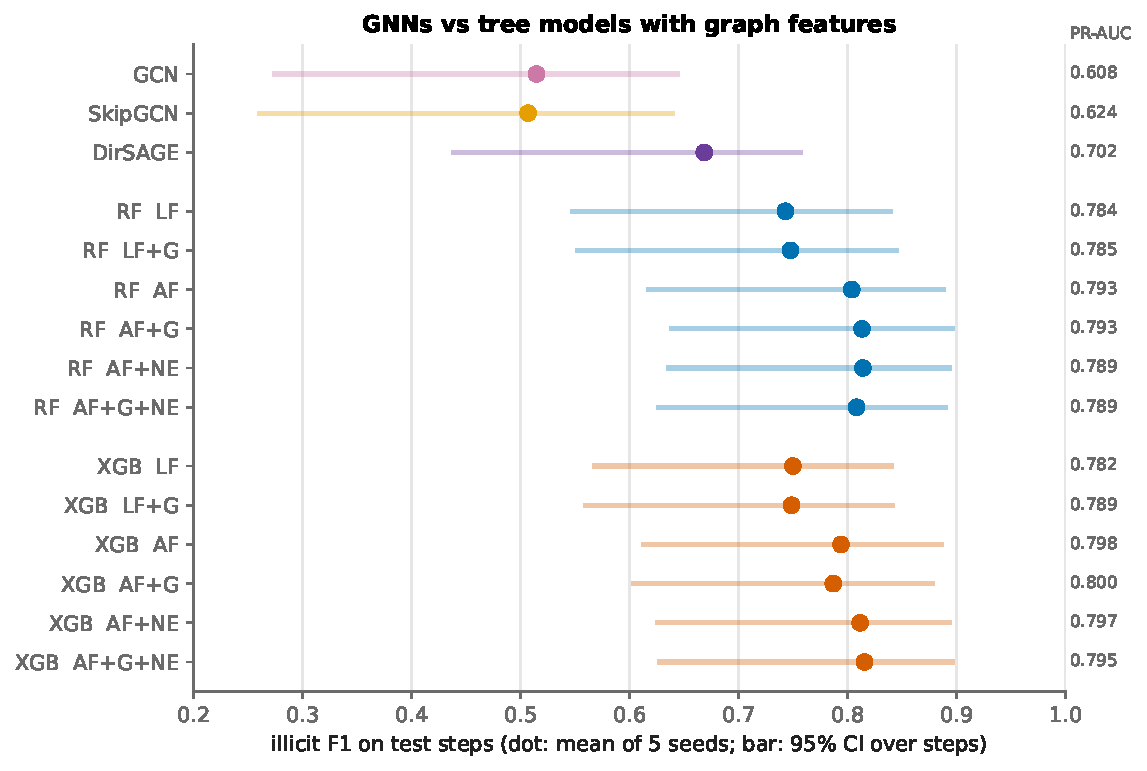
\includegraphics[width=\columnwidth]{../reports/figures/e04_graph.pdf}
  \caption{Illicit F1 of the graph neural networks and of the tree models on
  each feature set, with 95\% block-bootstrap intervals. Right: PR-AUC. LF local,
  AF all features, G structural graph features, NE GCN node embeddings.}
  \label{fig:graph}
\end{figure}

\subsection{Without labels (E6)}

The second angle of the project asked whether illicit transactions stand out
\emph{without} labels. The textbook approach, flagging the transactions an
Isolation Forest finds most anomalous, fails completely: PR-AUC
\IFAFUnsupAnomalousPRAUC{} and ROC-AUC \IFAFUnsupAnomalousROCAUC{}, worse than a
random ranking (PR-AUC \UnsBaseRate{}). The anomalies in this network are licit:
all of the 500 most anomalous labelled test transactions are licit, and they are
better connected than average (median degree 5 against 2). Illicit transactions
are \emph{typical} (Fig.~\ref{fig:anomaly}): they look like the bulk of ordinary
payments, consistent with their simple shape (at most three outputs,
Section~3). Fitting the forest on known licit transactions only does not change
this.

Inverting the rule, flagging the \emph{most typical} transactions, turns the same
forest into a useful detector: PR-AUC \IFAFUnsupTypicalPRAUC{} and ROC-AUC
\IFAFUnsupTypicalROCAUC{}, still with no label used for fitting. The direction is
one bit of domain knowledge, and it is the opposite of the usual assumption.

\begin{figure}[t]
  \centering
  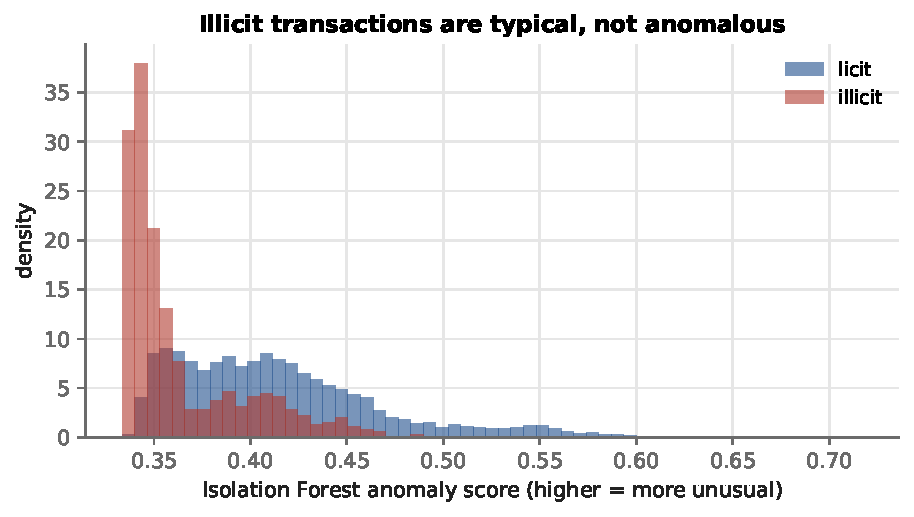
\includegraphics[width=\columnwidth]{../reports/figures/e06_anomaly_scores.pdf}
  \caption{Isolation Forest anomaly scores of labelled test transactions.
  Illicit transactions sit at the \emph{least} anomalous end.}
  \label{fig:anomaly}
\end{figure}

How many labels are worth more than that bit of knowledge?
Fig.~\ref{fig:labeleff} trains XGBoost on random subsets of the labelled training
data. With \LabelEffNA{} or \LabelEffNB{} labels it is below the label-free
detector; from about \LabelsToBeatIF{} labels on it is above it. With
\LabelEffNE{} labels it reaches \LabelEffE{}, and the remaining 29,000 labels add
less than 0.1 PR-AUC (\LabelsFullPRAUC{} with all of them). Labels are very
valuable at first and then quickly saturate. Better labels \emph{of the right
period} would help more than more labels (Section~\ref{sec:drift}).

\begin{figure}[t]
  \centering
  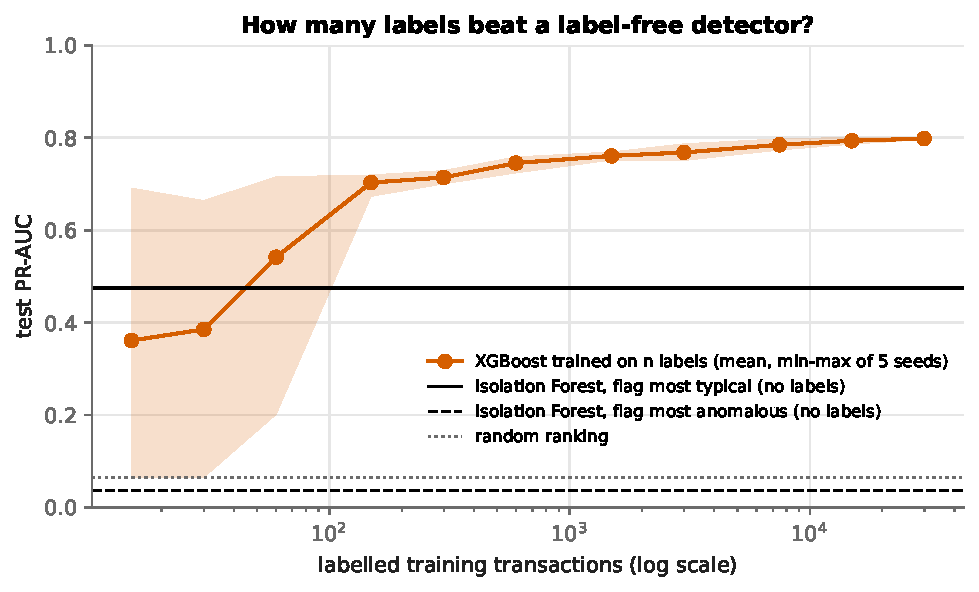
\includegraphics[width=\columnwidth]{../reports/figures/e06_label_efficiency.pdf}
  \caption{Test PR-AUC of XGBoost trained on $n$ random labelled transactions,
  against two label-free Isolation Forest rules.}
  \label{fig:labeleff}
\end{figure}

\subsection{What the model relies on (E8)}

SHAP values~\cite{lundberg2017} of XGBoost trained on AF+G attribute
\ShapLocal{} of the total importance to the 93 local features, \ShapAgg{} to the
72 aggregated ones and \ShapStruct{} to the nine structural features
(Fig.~\ref{fig:importance}). Shuffling each group on the test set confirms the
order and sharpens it: PR-AUC drops by \PermLocal{} without the local features,
\PermAggregated{} without the aggregated ones and \PermStructure{} without the
structure. The aggregated features get a large SHAP share but are partly
redundant with the local ones (correlation, Section~3); the model can fall back
on local information when they are shuffled, but not the other way round. The
group shares are the same before and after the shutdown, so the model does not
switch to different evidence when it starts to fail.

\begin{figure*}[t]
  \centering
  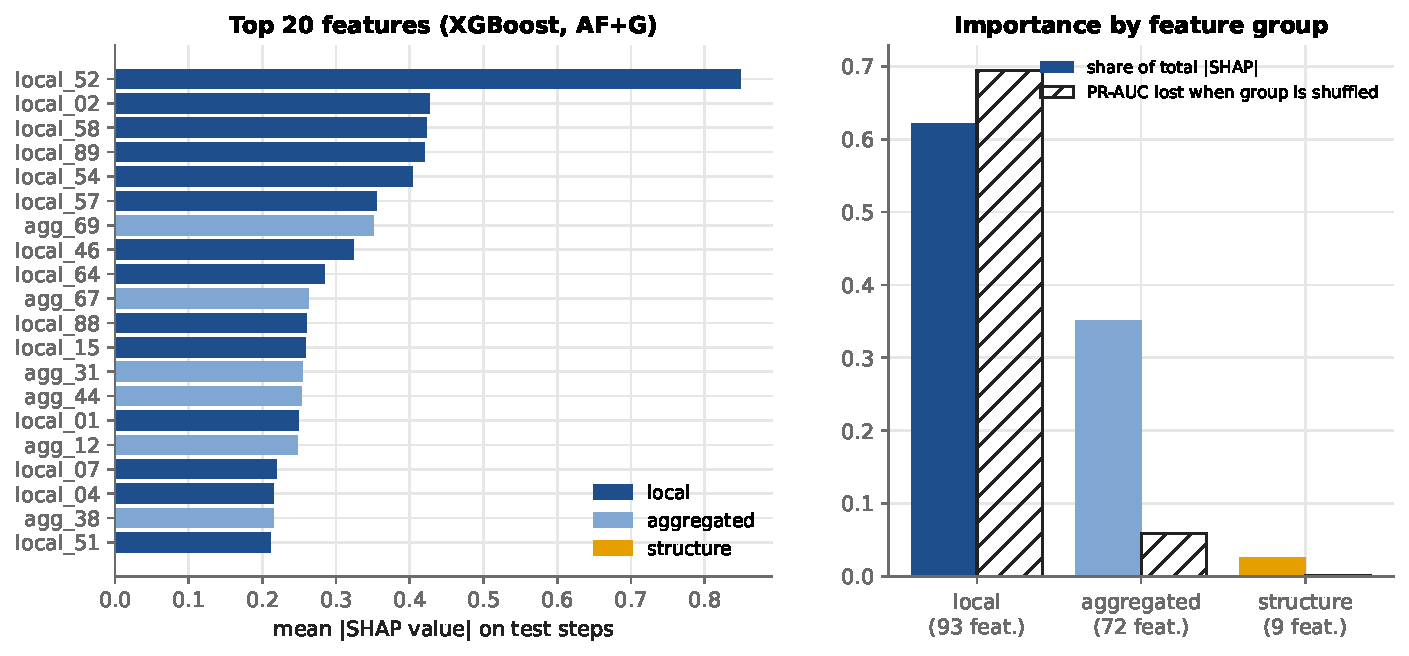
\includegraphics[width=0.85\textwidth]{../reports/figures/e08_importance.pdf}
  \caption{Left: the 20 features with the largest mean $|$SHAP$|$ (XGBoost,
  AF+G). Right: importance per feature group, as a share of total $|$SHAP$|$ and
  as the PR-AUC lost when the whole group is shuffled.}
  \label{fig:importance}
\end{figure*}

\subsection{Why performance collapses over time (E7)}
\label{sec:drift}

\begin{figure}[t]
  \centering
  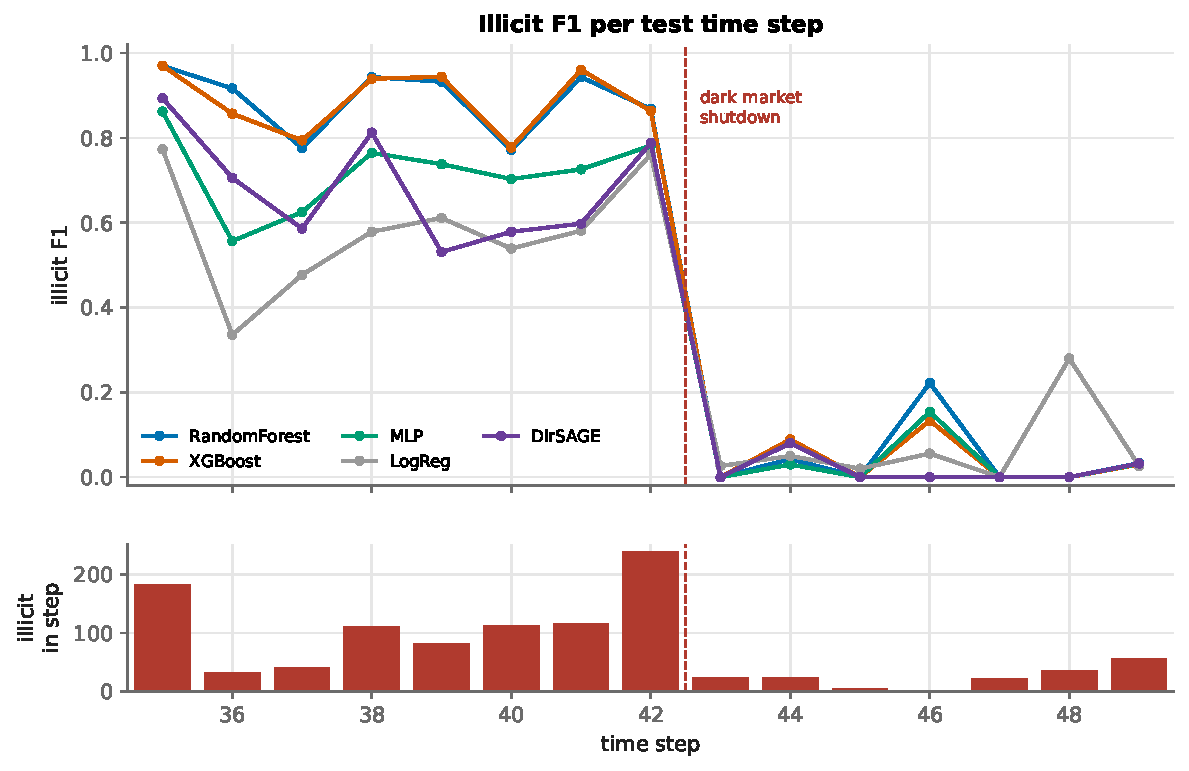
\includegraphics[width=\columnwidth]{../reports/figures/e07_f1_per_step.pdf}
  \caption{Illicit F1 per test step (top) and number of illicit transactions per
  step (bottom). Every model collapses at the dark market shutdown.}
  \label{fig:perstep}
\end{figure}

Fig.~\ref{fig:perstep} is the most important figure of this study. Before the
dark market shutdown, the tree models reach a mean per-step F1 of
\DriftRFPre{} (Random Forest) and \DriftXGBPre{} (XGBoost); from step 43 on they
reach \DriftRFPost{} and \DriftXGBPost{}. No model, linear, tree, neural or
graph, survives the event. The pooled test F1 of about 0.8 is therefore an
average of two regimes: near-perfect detection of a known kind of crime, and
almost no detection of the kind that replaced it.

\textbf{A hidden clock.} Before asking what changed, we had to remove something
that changes for everyone. \ClockCount{} of the aggregated features
(\ClockList{}) rise almost monotonically with time ($|\rho|\geq\ClockMinRho{}$
with the time step on the training steps). They work like the time-step column we
removed: any two periods can be told apart through them. Removing them from the
models changes nothing (F1 difference \ClockAblRFFoneDiff{}, $p\ClockAblRFFoneP{}$
for Random Forest), so the trees do not exploit them, but they must be removed
before any drift analysis.

\textbf{The illicit population changed; the licit one barely did.} Without the
clock features, we compare each feature's distribution before and after step 43
with a Kolmogorov--Smirnov test, separately for each class. For illicit
transactions, \AdvIllicitKSShare{} of the features shift strongly (KS
statistic $>0.3$); for licit transactions, only \AdvLicitKSShare{}. A classifier
can still separate the two periods within either class (AUC
\AdvIllicitAUC{} and \AdvLicitAUC{}), because a few slowly drifting features
remain. So the per-feature view is the informative one: almost every illicit
feature moved, while the licit population stayed largely the same.

\textbf{The new illicit transactions look licit.} For each illicit test
transaction we compare the distance to its nearest illicit training transaction
with the distance to its nearest licit one (Fig.~\ref{fig:novelty}). Before the
shutdown, \NovelPre{} are closer to licit traffic; after it, \NovelPost{}. A
model that learned what illicit activity \emph{used to} look like has nothing to
recognise.

\begin{figure}[t]
  \centering
  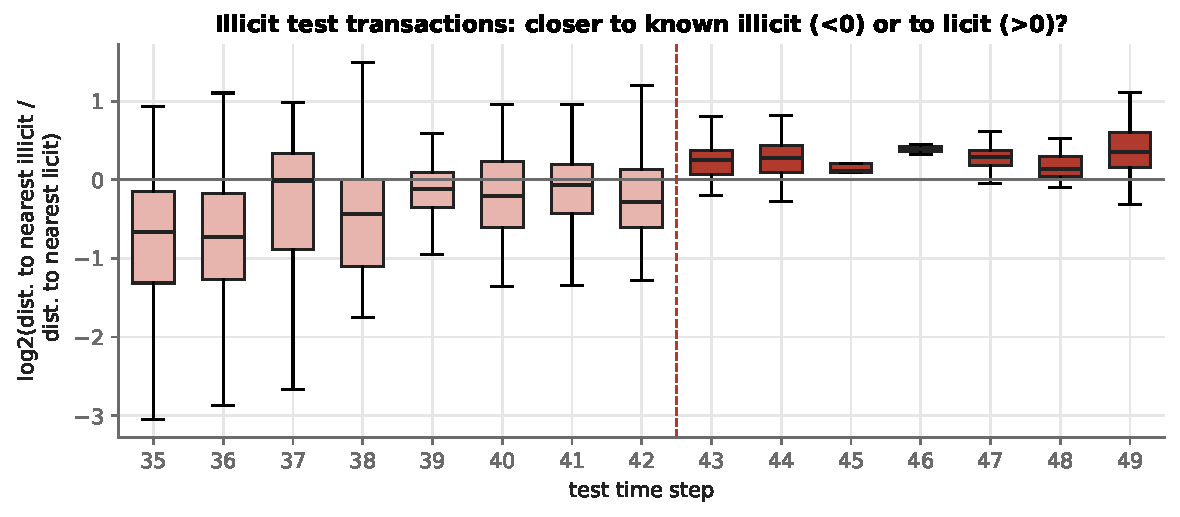
\includegraphics[width=\columnwidth]{../reports/figures/e07_novelty.pdf}
  \caption{Relative distance of illicit test transactions to the nearest
  illicit vs.\ nearest licit training transaction (log scale; above 0 means closer
  to licit). Clock features removed.}
  \label{fig:novelty}
\end{figure}

\textbf{Retraining helps only a little.} If the model is retrained on every
labelled step before scoring the next one (Fig.~\ref{fig:walk}), F1 after the
shutdown rises from \WFStaticPost{} to \WFExpandingPost{} (expanding window) or
\WFSlidingPost{} (last 10 steps), recovering mostly in the last step, once
enough new illicit examples have been labelled. Before the shutdown, retraining
changes little (\WFStaticPre{} vs \WFExpandingPre{}). This confirms and quantifies
the observation of Weber et al.: the bottleneck after a regime change is
labels for the new behaviour, not the model.

\begin{figure}[t]
  \centering
  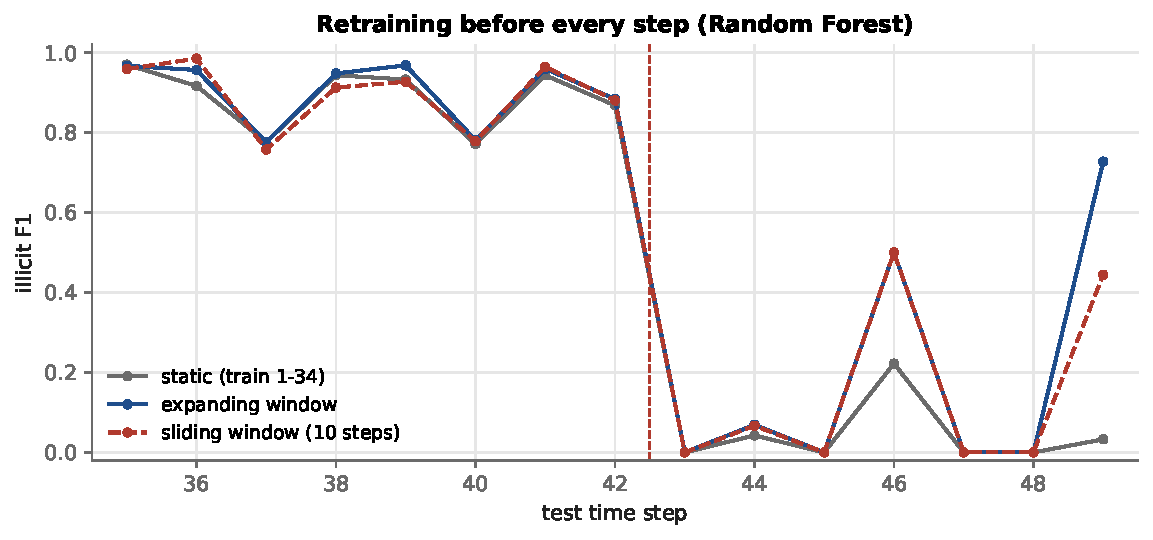
\includegraphics[width=\columnwidth]{../reports/figures/e07_walk_forward.pdf}
  \caption{Random Forest retrained before every test step on all earlier
  labelled steps (expanding) or the last 10 (sliding), vs.\ trained once.}
  \label{fig:walk}
\end{figure}

\section{Discussion}

\textbf{Answer to the research question.} Yes, illicit and licit transactions
can be told apart, with an illicit F1 around 0.8 and PR-AUC around 0.8 on unseen
future time steps, and the transaction graph helps. But almost all of the graph's
value is captured by the simplest summary: the features of a transaction's direct
neighbours. Learning from the graph end-to-end (GNNs), adding structural
statistics or adding GNN embeddings does not beat a tree ensemble on those
features. The one graph idea that clearly paid off was respecting the
\emph{direction} of payments, which lifted a GNN by about 0.15 F1.

\textbf{What a practitioner should take away.}
\begin{enumerate}
  \item \emph{Use a tree ensemble on local + neighbour features.} Random Forest
        and XGBoost are tied, strong and cheap. Neither needs re-balancing.
  \item \emph{Report uncertainty over time, not over rows.} With 15 test steps,
        the 95\% interval of F1 is about 0.27 wide. Most published differences on
        this benchmark are smaller than that.
  \item \emph{Do not assume crime is anomalous.} Here it is the opposite:
        illicit transactions are typical, and the anomalies are licit.
  \item \emph{Plan for regime changes, not for average performance.} After the
        dark market shutdown every model fails, retraining recovers little, and
        the new illicit transactions look like licit ones. Monitoring the score
        distribution and fast labelling of new cases matter more than model
        choice.
  \item \emph{Check embeddings for leakage.} A hybrid that feeds a tree with
        embeddings of a GNN trained on the same labels is only safe while the GNN
        is weak; out-of-fold embeddings are required otherwise.
\end{enumerate}

\textbf{Limitations.}
(i) The features are anonymised, so we cannot say \emph{what} the model learned
in domain terms, only which group of features it uses.
(ii) After step 43 there are only \EdaIllicitPost{} illicit test transactions,
and step 46 has almost none; per-step scores there are noisy.
(iii) The ``typical'' Isolation Forest needs one bit of prior knowledge (the
direction), which we only know from labelled data; on another network the
direction may differ.
(iv) We tuned each GNN over a small grid (four configurations); a larger search
or temporal GNNs such as EvolveGCN~\cite{pareja2020} might narrow the gap to the
tree models, though they did not in the original study.
(v) Labels come from Elliptic's heuristics and are themselves imperfect; 77\% of
transactions have none.

\textbf{Future work.} Semi-supervised use of the 157,205 unlabelled
transactions; drift detectors that raise an alarm when the score distribution
shifts, so retraining is triggered before performance is lost; and the richer
Elliptic++ data~\cite{elmougy2023}, which adds wallet-level information.

\section{Conclusion}

We reproduced the Elliptic benchmark, then rebuilt its evaluation so that no
choice depends on the test period and every claim carries a confidence interval.
Under this protocol, tree ensembles on local and neighbour features remain the
best detectors (F1 \MainRFFone{}, PR-AUC \MainXGBPRAUC{}); the graph helps through
neighbour aggregation, and directed message passing is the most effective GNN
design. Two results contradict common assumptions: illicit transactions are
\emph{less} anomalous than licit ones, and a better graph model can make a hybrid
\emph{worse}. Finally, we showed why every model fails after the dark market
shutdown: the illicit population changed in almost every feature and came to
resemble licit traffic. Detecting financial crime on a blockchain is less a
modelling problem than a problem of keeping up with a moving target.


\section*{Reproducibility}
Code, results, figures and this report are at
\url{https://github.com/berbicanes/EllipticML}. \texttt{make all} rebuilds every
number from the raw CSV files; \texttt{make report} regenerates
\texttt{numbers.tex} and compiles this document, so the results in the text and
tables are read from the results files rather than typed by hand. Unit tests
check the split for leakage.

\bibliographystyle{IEEEtran}
\bibliography{references}

\end{document}
